\section{Background}

\subsection{Problem Statement}

\begin{frame}{}
  \begin{center}
    Why is this not about ANNS anymore?
  \end{center}
\end{frame}

\begin{frame}{}
  \begin{definition}[Random Sampling without Replacement]
    Given a data set \(X\), we uniformly pick \(k\) elements
    from \(X\) such that none repeat.
  \end{definition}

  Use cases:
  \begin{itemize}
    \item Splitting train-test data for ML 
    \item Subsampling for efficiency
  \end{itemize}
\end{frame}

\begin{frame}{Work-Span Model for Cost Analysis}
  \begin{definition}[Work]
    The \textit{work}, often denoted by \(W\), of a parallel algorithm is the 
    total number of operations done in the whole computation.
  \end{definition}

  \begin{definition}[Span]
    The \textit{span}, often denoted by \(S\), of a parallel algorithm is the
    longest chain of dependencies in a computation DAG.
  \end{definition}
\end{frame}

\begin{frame}{Work-Span Model for Cost Analysis Example}
  \begin{algorithm}[H]
    \caption{ParComp}
    \begin{algorithmic}
      \State{Compute \(A\) and \(B\) in parallel}
      \State{Compute \(C\)}
    \end{algorithmic}
  \end{algorithm}
  
  \(A\), \(B\), and \(C\) takes \(a, b\), and \(c\) operations respectively.
  \begin{itemize}
    \item Work is \(a + b + c\)
    \item Span is \(\max(a, b) + c\)
  \end{itemize}
\end{frame}

\subsection{Existing Algorithms}

\begin{frame}{Baseline: Pick and Remove}
  \begin{algorithm}[H]
    \caption{\textsc{PickAndRemove}}
  \begin{algorithmic}
    \Input{Data set \(X\), Sample size \(k\)}
    \Output{Sample \(S\) with \(|S| = k\)}
    \For{\(i = 1, 2, \ldots, k\)}
      \State{Pick \(x\) u.a.r. from \(X\)}
      \State{Add \(x\) to \(S\)}
      \State{Remove \(x\) from \(X\)}
    \EndFor
    \State{\Return{\(S\)}}
  \end{algorithmic}
  \end{algorithm}

  Sequential running time of \(\O(n)\).
\end{frame}

\begin{frame}{Improvement 1: Priority Sampling}
  \begin{algorithm}[H]
    \caption{\textsc{PrioritySample}}
  \begin{algorithmic}
    \Input{Data set \(X\), Sample size \(k\)}
    \Output{Sample with size \(k\)}

    \State{Assign priority from \(\Unif(0, 1)\) to each element
    of \(X\)}
    \State{\Return{\textsc{QuickSelect(\(X, k\))} using priority for comparison}}
  \end{algorithmic}
  \end{algorithm}

  Sequential running time of \(\O(n)\) w.h.p.\footnote{Probability at least \(1 -
  n^{-c}\) for constant \(c > 0\)}
\end{frame}

\begin{frame}{Improvement 1': Priority Sampling}
  \begin{algorithm}[H]
    \caption{\textsc{ParPrioritySample}}
  \begin{algorithmic}
    \Input{Data set \(X\), Sample size \(k\)}
    \Output{Sample with size \(k\)}

    \State{Assign priority from \(\Unif(0, 1)\) to each element
    of \(X\) in parallel}
    \State{\Return{\textsc{ParQuickSelect(\(X, k\))} using priority for comparison}}
  \end{algorithmic}
  \end{algorithm}

  Work is \(\O(n)\) and span is \(\O(\log^2 n)\) w.h.p.

  Performs pretty well when \(k \approx n\).
\end{frame}

% \begin{frame}{Recap: Quick Select}
%   \begin{algorithm}[H]
%     \caption{\textsc{QuickSelect}}
%   \begin{algorithmic}
%     \Input{Data set \(Y\), Sample size \(l\)}
%     \Output{Sample with size \(l\)}
%
%     \State{Pick \(p\) u.a.r. from \(Y\)}
%     \State{\(LE \gets\) elements of \(Y\) less than or equals to \(p\)}
%     \State{\(G \gets\) elements of \(Y\) greater than \(p\)}
%
%     \IIf{\(|LE| = k\)}{\Return{\(LE\)}}
%     \IElsIf{\(|LE| > k\)}{\Return{\textsc{QuickSelect(\(LE, l\))}}}
%     \IElse{\Return{\textsc{Concat(\(LE\), QuickSelect(\(G,
%     l - |LE|\)))}}}
%   \end{algorithmic}
%   \end{algorithm}
%
%   The parallel variant constructs \(LE\) \(G\) in parallel.
% \end{frame}

\begin{frame}{Improvement 2: Permutation Sampling}
  \begin{algorithm}[H]
    \caption{\textsc{PermutationSample}}
  \begin{algorithmic}
    \Input{Data set \(X\), Sample size \(k\)}
    \Output{Sample with size \(k\)}

    \State{Generate swap target \(H\) such that \(i \leq H[i] \leq n\)}
    \State{\textsc{Permute(\(X, H\))}}
    \State{\Return{\(X[{}:k]\)}}
  \end{algorithmic}
  \end{algorithm}
  \vspace{-1em}
  \begin{algorithm}[H]
    \caption{\textsc{Permute} or Knuth Shuffle via Fisher-Yates}
  \begin{algorithmic}
    \Input{Data set \(X\), Swap target \(H\)}
    \For{\(i = 1, 2, \ldots, n\)}
      \State{\textsc{Swap(\(A[i], A[H[i]]\))}}
    \EndFor
  \end{algorithmic}
  \end{algorithm}
\end{frame}

\begin{frame}{Can we do better?}
  So far, existing algorithms run in \(\O(n)\)
  \begin{enumerate}
    \item When \(k \approx n\), doesn't really matter
    \item When \(k \ll n\), does too much work
  \end{enumerate}

  This project focuses on tackling the second case using Permutation Sampling.
\end{frame}

\subsection{Improvements via Permutation Sampling}

\begin{frame}{Knuth Shuffle}
  Issue 1: \textsc{Permute} is super sequential!

  \begin{algorithm}[H]
    \caption{\textsc{Permute} or Knuth Shuffle via Fisher-Yates}
    \begin{algorithmic}
      \Input{Data set \(X\), Swap target \(H\)}
      \For{\(i = 1, 2, \ldots, n\)}
        \State{\textsc{Swap(\(A[i], A[H[i]]\))}}
      \EndFor
    \end{algorithmic}
  \end{algorithm}
\end{frame}

\begin{frame}{Parallel Knuth Shuffle}
  According to Shun et al. \cite{julian-parperm}, you can run Knuth Shuffle in
  parallel.

  \begin{figure}[ht]
    \begin{center}
      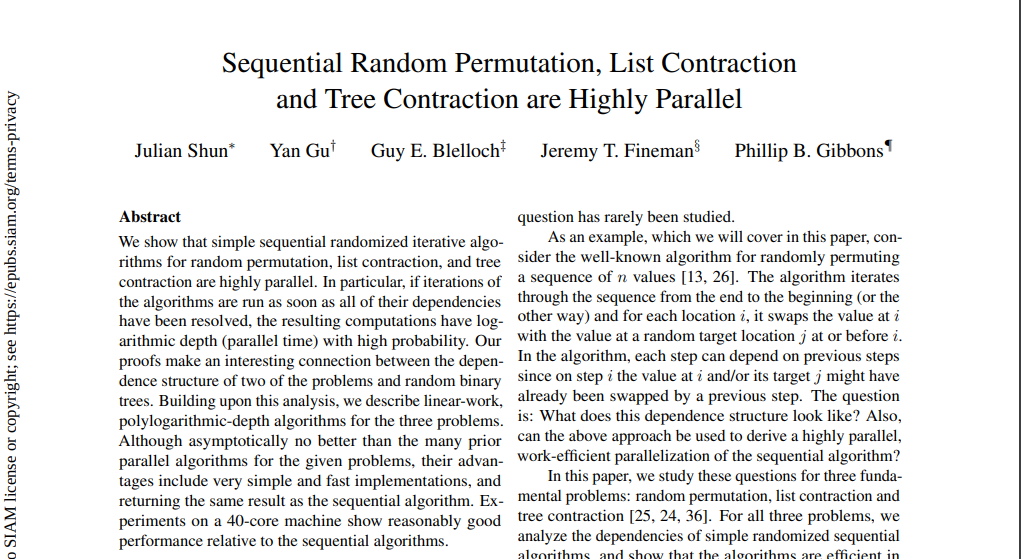
\includegraphics[width=0.60\textwidth]{julian-paper}
    \end{center}
    \caption{Shun et al. \cite{julian-parperm}}
  \end{figure}
\end{frame}

\begin{frame}{Parallel Knuth Shuffle}
  Useful results:
  \begin{enumerate}
    \item Swap target \(H\) can be converted into a Dependency DAG resembling a random BT
    \item \(\O(1)\) \textit{readiness} detection gives \(\O(n)\) work and
      \(\O(\log n)\) span for Knuth Shuffle w.h.p.
    \item Parallel and sequential Knuth Shuffle gives same output
  \end{enumerate}
\end{frame}

\begin{frame}{Parallel Knuth Shuffle --- Result 1: Turn \(H\) into DDAG}
  \begin{figure}
    \hfill
    \begin{subfigure}{0.3\textwidth}
      \centering
      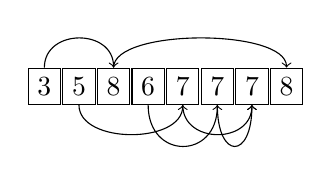
\begin{tikzpicture}[
        arr-elm/.style = {draw, rectangle, text centered, minimum size=0.5em}, 
        node distance = 1.25em
      ]
        \node[arr-elm] (1) {3};
        \node[arr-elm,right of=1] (2) {5};
        \node[arr-elm,right of=2] (3) {8};
        \node[arr-elm,right of=3] (4) {6};
        \node[arr-elm,right of=4] (5) {7};
        \node[arr-elm,right of=5] (6) {7};
        \node[arr-elm,right of=6] (7) {7};
        \node[arr-elm,right of=7] (8) {8};

        \draw[->] (1.north) .. controls +(up:5mm) and +(up:5mm) .. (3.north);
        \draw[->] (3.north) .. controls +(up:5mm) and +(up:5mm) .. (8.north);

        \draw[->] (2.south) .. controls +(down:5mm) and +(down:5mm) .. (5.south);
        \draw[->] (5.south) .. controls +(down:5mm) and +(down:5mm) .. (7.south);

        \draw[->] (4.south) .. controls +(down:7mm) and +(down:7mm) .. (6.south);
        \draw[->] (6.south) .. controls +(down:7mm) and +(down:7mm) .. (7.south);
      \end{tikzpicture}
      \caption{Dependency of \(H\)}
    \end{subfigure}
    \hfill
    \begin{subfigure}{0.3\textwidth}
      \centering
      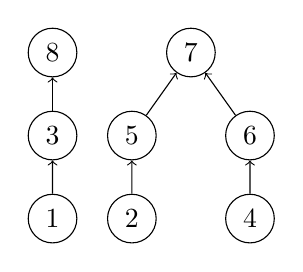
\begin{tikzpicture}[
          vtx/.style = {draw, circle},
          edge from parent/.style = {draw,<-},
          level/.style = {level distance = 3em},
          node distance = 5em,
        ]
        \node[vtx] (8) {8} child { node[vtx] {3} child { node[vtx] {1} } };
        \node[vtx,right of=8] {7} 
          child { node[vtx] {5} child { node[vtx] {2} }}
          child { node[vtx] {6} child { node[vtx] {4} }};
      \end{tikzpicture}
      \caption{Extracted into a forest}
    \end{subfigure}
    \hfill
    \begin{subfigure}{0.3\textwidth}
      \centering
      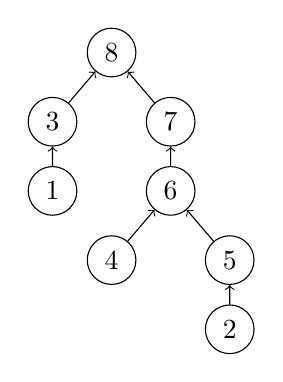
\begin{tikzpicture}[
        vtx/.style = {draw, circle},
        edge from parent/.style = {draw,<-},
        level/.style = {level distance = 2.5em},
        node distance = 5em,
      ]
        \node[vtx] (8) {8} 
          child { node[vtx] {3} child { node[vtx] {1} } }
          child { node[vtx] {7} 
            child { node[vtx] {6} child { node[vtx] {4} }
              child { node[vtx] {5} child { node[vtx] {2} }}
            }
          };
      \end{tikzpicture}
      \caption{Modified into DDAG}
    \end{subfigure}
    \hfill
    \caption{DDAG constructed from \(H = [
      \underset{1}{3}, 
      \underset{2}{5}, 
      \underset{3}{8}, 
      \underset{4}{6}, 
      \underset{5}{7}, 
      \underset{6}{7}, 
      \underset{7}{7}, 
      \underset{8}{8} 
    ]\)}
  \end{figure}
\end{frame}

\begin{frame}{Parallel Knuth Shuffle --- Result 2: Constant Readiness Detection}
  \begin{definition}[Ready]
    Step \(i\) is said to be \textit{ready} if every step that
    points to \(i\) in the DDAG has been processed.
  \end{definition}

  \begin{columns}
    \begin{column}{0.4\textwidth}
      \begin{figure}[ht]
        \centering
        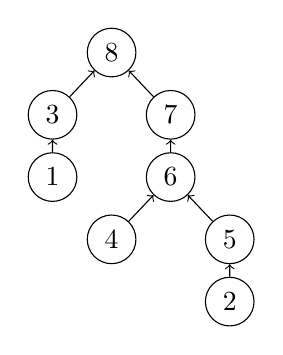
\begin{tikzpicture}[
            vtx/.style = {draw, circle},
            edge from parent/.style = {draw,<-},
            level/.style = {level distance = 2.25em},
          ]
          \node[vtx] (8) {8} 
            child { node[vtx] {3} child { node[vtx] {1} } }
            child { node[vtx] {7} 
              child { node[vtx] {6} child { node[vtx] {4} }
                child { node[vtx] {5} child { node[vtx] {2} }}
              }
            };
        \end{tikzpicture}
        \caption{\(H = [
          \underset{1}{3}, 
          \underset{2}{5}, 
          \underset{3}{8}, 
          \underset{4}{6}, 
          \underset{5}{7}, 
          \underset{6}{7}, 
          \underset{7}{7}, 
          \underset{8}{8} 
        ]\)}
      \end{figure}
    \end{column}
    \hfill
    \begin{column}{0.6\textwidth}
      \begin{itemize}
        \item 8 is ready once 3 and 7 processed
        \item 3 is ready once 1 processed
        \item 7 is ready once 6 processed
        \item 6 is ready once 4 and 5 processed
      \end{itemize}
    \end{column}
  \end{columns}
\end{frame}

\begin{frame}{Parallel Knuth Shuffle --- Result 2: Constant Readiness Detection}
  \begin{columns}
    \begin{column}{0.4\textwidth}
      \begin{figure}[ht]
        \centering
        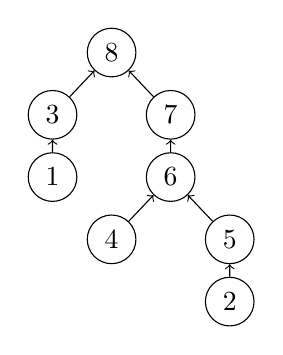
\begin{tikzpicture}[
            vtx/.style = {draw, circle},
            edge from parent/.style = {draw,<-},
            level/.style = {level distance = 2.25em},
          ]
          \node[vtx] (8) {8} 
            child { node[vtx] {3} child { node[vtx] {1} } }
            child { node[vtx] {7} 
              child { node[vtx] {6} child { node[vtx] {4} }
                child { node[vtx] {5} child { node[vtx] {2} }}
              }
            };
        \end{tikzpicture}
        \caption{\(H = [
          \underset{1}{3}, 
          \underset{2}{5}, 
          \underset{3}{8}, 
          \underset{4}{6}, 
          \underset{5}{7}, 
          \underset{6}{7}, 
          \underset{7}{7}, 
          \underset{8}{8} 
        ]\)}
      \end{figure}
    \end{column}
    \hfill
    \begin{column}{0.6\textwidth}
      \# readiness checks for step \(i\) is height in DDAG
      \begin{itemize}
        \item Keep checking until ready
        \item After ready, process, and never check again
      \end{itemize}
    \end{column}
  \end{columns}
\end{frame}

\begin{frame}{Parallel Knuth Shuffle --- Result 2: Constant Readiness Detection}
  We know:
  \begin{itemize}
    \item \# readiness checks for step \(i\) is height in DDAG
    \item Height of DDAG is \(\O(\log n)\) w.h.p. \cite{julian-parperm}
  \end{itemize}

  Implications if readiness check is \(\O(1)\):
  \begin{itemize}
    \item Span is \(\O(\log n)\) w.h.p. since can check level in parallel
    \item Work is \(\O(n)\) in expectation since computed from sum of all heights
  \end{itemize}
\end{frame}

\begin{frame}{Parallel Knuth Shuffle --- Result 3: Par. and Seq. have Same Output}
  \begin{columns}
    \begin{column}{0.45\textwidth}
      \begin{figure}
        \centering
        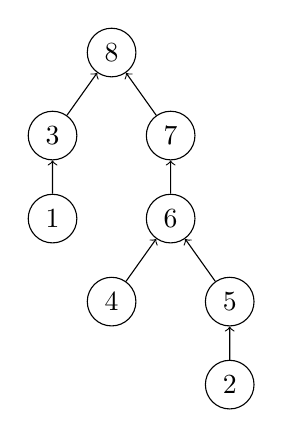
\begin{tikzpicture}[
          vtx/.style = {draw, circle},
          edge from parent/.style = {draw,<-},
          level/.style = {level distance = 3em},
          node distance = 5em,
        ]
          \node[vtx] (8) {8} 
            child { node[vtx] {3} child { node[vtx] {1} } }
            child { node[vtx] {7} 
              child { node[vtx] {6} child { node[vtx] {4} }
                child { node[vtx] {5} child { node[vtx] {2} }}
              }
            };
        \end{tikzpicture}
        \caption{\(H = [
          \underset{1}{3}, 
          \underset{2}{5}, 
          \underset{3}{8}, 
          \underset{4}{6}, 
          \underset{5}{7}, 
          \underset{6}{7}, 
          \underset{7}{7}, 
          \underset{8}{8} 
        ]\)}
      \end{figure}
    \end{column}
    \begin{column}{0.5\textwidth}
      Observation: 
      \begin{itemize}
        \item Leaf-to-root path is ascending
        \item Order of swapping are the same
      \end{itemize}
    \end{column}
  \end{columns}
\end{frame}

\begin{frame}{Parallel Knuth Shuffle --- Implementation}
  \textit{Deterministic Reservation} is a framework by Blelloch et al. 
  \cite{blelloch-detreserve}
  \begin{itemize}
    \item For parallel algorithms whose DDAG is
      unique for each input under fork-join
      \begin{itemize}
        \item \textsc{MergeSort} has only one DDAG for one input
        \item \textsc{QuickSort} could have multiple DDAG for one input
          input
      \end{itemize}
    \item Ensure determinism despite different CPU scheduling
    \item Splits processing round into 2 phases: Reservation and Committing
  \end{itemize}
\end{frame}

\begin{frame}{Parallel Knuth Shuffle --- Implementation}
  Primitive from deterministic reservation: \textsc{WriteMin(\(l, x\))}
  \begin{algorithm}[H]
    \caption{\textsc{WriteMin}}
    \begin{algorithmic}
      \Input{Memory address \(l\), New value \(x\)}
      \State{\(DRAM[l] \gets \min(DRAM[l], x)\)}
    \end{algorithmic}
  \end{algorithm}

  \begin{itemize}
    \item Could cause race condition
    \item Use atomic types
  \end{itemize}
\end{frame}

\begin{frame}{Parallel Knuth Shuffle --- Implementation}
  \begin{algorithm}[H]
    \caption{\textsc{Reserve}}
    \begin{algorithmic}
      \Input{Reservation array \(R\), Swap targets \(H\), Index \(i\)}
      \State{\textsc{WriteMin(\(R[i], i\))}}
      \State{\textsc{WriteMin(\(R[H[i]], i\))}}
    \end{algorithmic}
  \end{algorithm}
  \vspace{-1.5em}
  \begin{algorithm}[H]
    \caption{\textsc{Commit}}
    \begin{algorithmic}
      \Input{Reservation array \(R\), Swap targets \(H\), Index \(i\)}
      \Output{0 if swap happened and 1 otherwise}
      \If{\(R[i] = R[H[i]] = i\)}
        \State{\textsc{Swap(\(A[i], A[H[i]]\))}}
        \State{\Return 0}
      \EndIf
      \State{\Return 1}
    \end{algorithmic}
  \end{algorithm}
\end{frame}

\begin{frame}{Parallel Knuth Shuffle --- Implementation}
  During reservation phase, we run
  \begin{itemize}
    \item \textsc{Reserve(\(R[5], 5\))} then \textsc{Reserve(\(R[7], 5\))}
    \item \textsc{Reserve(\(R[6], 6\))} then \textsc{Reserve(\(R[7], 6\))}
  \end{itemize}
  Resulting in:
  \begin{figure}
    \centering
    \begin{tikzpicture}[
      arr-elm/.style = {draw, rectangle, text centered, minimum size=1.5em}, 
      node distance = 1.5em
    ]
      % H
      \node[arr-elm,fill=Processed] (1) {3};
      \node[arr-elm,right of=1,fill=Processed] (2) {5};
      \node[arr-elm,right of=2,fill=Processed] (3) {8};
      \node[arr-elm,right of=3,fill=Processed] (4) {6};
      \node[arr-elm,right of=4,fill=Processing] (5) {7};
      \node[arr-elm,right of=5,fill=Processing] (6) {7};
      \node[arr-elm,right of=6,fill=Processing] (7) {7};
      \node[arr-elm,right of=7] (8) {8};
      \node[left of=1,node distance=2em] (hh) {\(H\):};

      \draw[->] (5.south) .. controls +(down:5mm) and +(down:5mm) .. (7.south);
      \draw[->] (6.north) .. controls +(up:5mm) and +(up:5mm) .. (7.north);

      % R
      \node[arr-elm,below of=1,node distance=3em] (1r) {\(*\)};
      \node[arr-elm,right of=1r] (2r) {\(*\)};
      \node[arr-elm,right of=2r] (3r) {\(*\)};
      \node[arr-elm,right of=3r] (4r) {\(*\)};
      \node[arr-elm,right of=4r] (5r) {5};
      \node[arr-elm,right of=5r] (6r) {6};
      \node[arr-elm,right of=6r] (7r) {5};
      \node[arr-elm,right of=7r] (8r) {\(*\)};
      \node[left of=1r,node distance=2em] (rr) {\(R\):};
    \end{tikzpicture}
  \end{figure}
  \(\therefore\) swap \(A[5]\) and \(A[7]\) during commit
\end{frame}

\begin{frame}{Parallel Knuth Shuffle}
  \begin{algorithm}[H]
    \caption{\textsc{ParPermute}}
    \begin{algorithmic}
      \Input{Array \(A\), Swap targets \(H\)}

      \State{\(I \gets [1, 2, \ldots, n]\)} \Comment{unprocessed indices}
      \State{\(R \gets [n, n, \ldots, n]\) of length \(n\)} \Comment{reservation slot}
      \While{\(I\) is not empty}
        \ParFor{\(i \in I\)} \Comment{only prefix of \(I\) in practice}
          \State{\textsc{Reserve(\(R, i\))}}
        \EndParFor
        \ParFor{\(i \in I\)}
          \State{\textsc{Commit(\(R, i\))}}
        \EndParFor
        \State{Remove committed indices from \(I\)}
      \EndWhile
    \end{algorithmic}
  \end{algorithm}
\end{frame}

\begin{frame}{Parallel Knuth Shuffle --- Implementation}
  \begin{figure}
    \centering
    \begin{tikzpicture}[
      arr-elm/.style = {draw, rectangle, text centered, minimum size=1.5em}, 
      node distance = 1.5em
    ]
      \node[arr-elm] (8) {8};
      \node[arr-elm,left of=8] (7) {7};
      \node[arr-elm,left of=7] (6) {7};
      \node[arr-elm,left of=6] (5) {7};
      \node[arr-elm,left of=5] (4) {6};
      \node[arr-elm,left of=4,fill=Processing] (3) {8};
      \node[arr-elm,left of=3,fill=Processing] (2) {5};
      \node[arr-elm,left of=2,fill=Processing] (1) {3};
      \draw[->] (1.north) .. controls +(up:5mm) and +(up:5mm) .. (3.north);
      \draw[->] (2.north) .. controls +(up:7mm) and +(up:7mm) .. (5.north);
      \draw[->] (3.north) .. controls +(up:5mm) and +(up:5mm) .. (8.north);
      \node[anchor=west,text width=20em,left of=1,node distance=15em] (op1) {Execute \textsc{Swap(1,3)}, \textsc{Swap(2,5)}};

      \node[arr-elm,below of=8,node distance=4em] (82) {8};
      \node[arr-elm,left of=82] (72) {7};
      \node[arr-elm,left of=72] (62) {7};
      \node[arr-elm,left of=62,fill=Processing] (52) {7};
      \node[arr-elm,left of=52,fill=Processing] (42) {6};
      \node[arr-elm,left of=42,fill=Processing] (32) {8};
      \draw[->] (32.north) .. controls +(up:9mm) and +(up:9mm) .. (82.north);
      \draw[->] (42.north) .. controls +(up:7mm) and +(up:7mm) .. (62.north);
      \draw[->] (52.north) .. controls +(up:5mm) and +(up:5mm) .. (72.north);
      \node[anchor=west,text width=20em,below of=op1,node distance=4em] (op2) {Execute \textsc{Swap(3,8)}, \textsc{Swap(4,6)}, \textsc{Swap(5,7)}};

      \node[arr-elm,below of=82,node distance=4em,fill=Processing] (83) {8};
      \node[arr-elm,left of=83,fill=Processing] (73) {7};
      \node[arr-elm,left of=73,fill=Processing] (63) {7};
      \draw[->] (63.north) .. controls +(up:5mm) and +(up:5mm) .. (73.north);
      \draw[->] (73.south west) .. controls +(down:5mm) and +(down:5mm) .. (73.south);
      \draw[->] (83.north) .. controls +(up:7mm) and +(right:7mm) .. (83.east);
      \node[anchor=west,text width=20em,below of=op2,node distance=4em] (op3) {Execute \textsc{Swap(6,7)}, \textsc{Swap(8,8)}};

      \node[arr-elm,below of=73,node distance=4em,fill=Processing] (74) {7};
      \draw[->] (74.north) .. controls +(up:7mm) and +(right:7mm) .. (74.east);
      \node[anchor=west,text width=20em,below of=op3,node distance=4em] (op4) {Execute \textsc{Swap(7,7)}};
    \end{tikzpicture}
  \end{figure}
\end{frame}
